\documentclass[../AnalisideiRequisiti.tex]{subfiles}

\begin{document}
	
\chapter{Descrizione generale}

\section{Obiettivo del prodotto}

Lo scopo del progetto consiste nel creare un applicativo software di supporto allo sviluppo di \glossario{Speect}{Speect}. L’applicazione da creare è una interfaccia grafica che aiuti i programmatori nello sviluppo dei plug-in per Speect. Nell’interfaccia utente si deve poter visualizzare e modificare i grafi delle \glossario{utterance}{utterance} di Speect. 


\section{Funzioni del prodotto}
L’interfaccia grafica permetterà di:
\begin{itemize}
	\item{} Caricare i \glossario{file .json}{file .json} utili all’inizializzazione di Speect;
	\item{} Mostrare i grafi delle varie utterance;
	\item{} Aggiunta, modifica e eliminazione degli archi dei nodi;
	\item{} La modifica dei campi dei nodi;
	\item{} Disporre graficamente i nodi per permettere una lettura semplificata;
	\item{} Ritornare il file audio generato da Speect;
	\item{} Permettere una stampa grafica dei grafi;
	\item{} Poter visualizzare passo passo i grafi delle varie utterance in modo sequenziale, cioè l’utente potrà decidere quando eseguire e visualizzare il grafo della successiva utterance.	
\end{itemize}


\section{Caratteristiche degli utenti}
Il software si rivolge a programmatori esperti che si occupano di sviluppare plug-in per Speect. L'utente deve possedere una buona conoscenza di Speect e delle sue componenti.

\section{Piattaforma di esecuzione}
Sarà possibile eseguire il software su tutte le macchine desktop con sistema operativo Linux, dovranno essere presenti \glossario{CMAKE}{CMAKE}, \glossario{GCC}{GCC} e le librerie di \glossario{QT}{QT}. Verranno comunque utilizzate tecnologie presenti anche su sistemi Windows in questo modo sarà possibile la compilazione, però non verrà fornito un manuale di installazione per quest’ultima piattaforma.

\section{Vincoli generali}
Il software realizzato dovrà rispettare vari requisiti:
\begin{itemize}
	\item{} Requisiti obbligatori:
	\begin{itemize}
		\item{}Realizzazione di una interfaccia grafica per Speect in grado di:
		\begin{enumerate}
			\item{} Caricare un \glossario{file Voice}{file Voice} con estensione JSON;
			\item{} Inserire un input di testo, che verrà utilizzato in fase di compilazione;
			\item{} Selezionare il tipo di \glossario{utterance type}{utterance type} di compilazione;
			\item{} Compilazione mediante Speect dato input di testo e l'utterance type;
			\item{} Visualizzazione grafica del grafo prodotto dalla compilazione;
			\item{} Spostare un nodo graficamente;
			\item{} Selezionato un nodo dall'interfaccia grafica, visualizzare le informazioni del nodo;
			\item{} Possibilità di salvare un file audio con estensione \glossario{WAV}{WAV} generato a seguito di una compilazione di Speect.
		\end{enumerate}
		\item{}	Documentazione tecnica del software;
	\end{itemize}
	\item{} Requisiti desiderabili:
	\begin{itemize}
		\item{} Selezione file JSon tramite \glossario{Drag and Drop}{drag and drop}
		\item{} Permettere all'utente di selezionare le relazioni del grafo da visualizzare;
		\item{} Permettere la riproduzione del file audio prodotto;
		\item{} Permettere di nascondere i nodi senza dati;
		\item{} Cambiare il colore degli strati del grafo.
	\end{itemize}
	\item{} Requisiti facoltativo:
	\begin{itemize}
		\item{} Evidenziare un nodo dato un percorso riferito al grafo;
		\item{} Poter eseguire passo passo le varie utterance;
		\item{}	Modificare gli archi che collegano i vari nodi dei grafi delle utterance;
		\item{} Caricare e salvare lo stato di un grafo precedentemente realizzato;
		\item{} Poter compilare partendo da un grafo caricato;
		\item{}	Possibilità di confrontare visivamente due stati della struttura interna di Speect;
		\item{} Possibilità di confrontare automaticamente due stati della struttura interna di Speect;
		\item{} Modificare il file Voice di estensione JSON caricato nell'applicazione.
	\end{itemize}
	
\end{itemize}

\chapter{Interfaccia Grafica}
In questa parte verrà presentato, in linea generale, il funzionamento dell'interfaccia grafica. Le interfacce proposte nelle immagini che seguono non rappresentano le finestre che saranno implementare, ma semplicemente vogliono essere una linea guida per comprendere al meglio le varie funzionalità dell'applicazione; quindi l'estetica di \textit{\glossario{DeSpeect}{DeSpeect}} potrebbe differire dalle immagini che seguono. Le istruzioni che seguono non intendono essere in alcun modo una guida all'utilizzo dell'applicazione.


	\section{Schermata principale}
		\begin{figure}[htp]
			\caption{Esempio pagina principale}
			\centering
			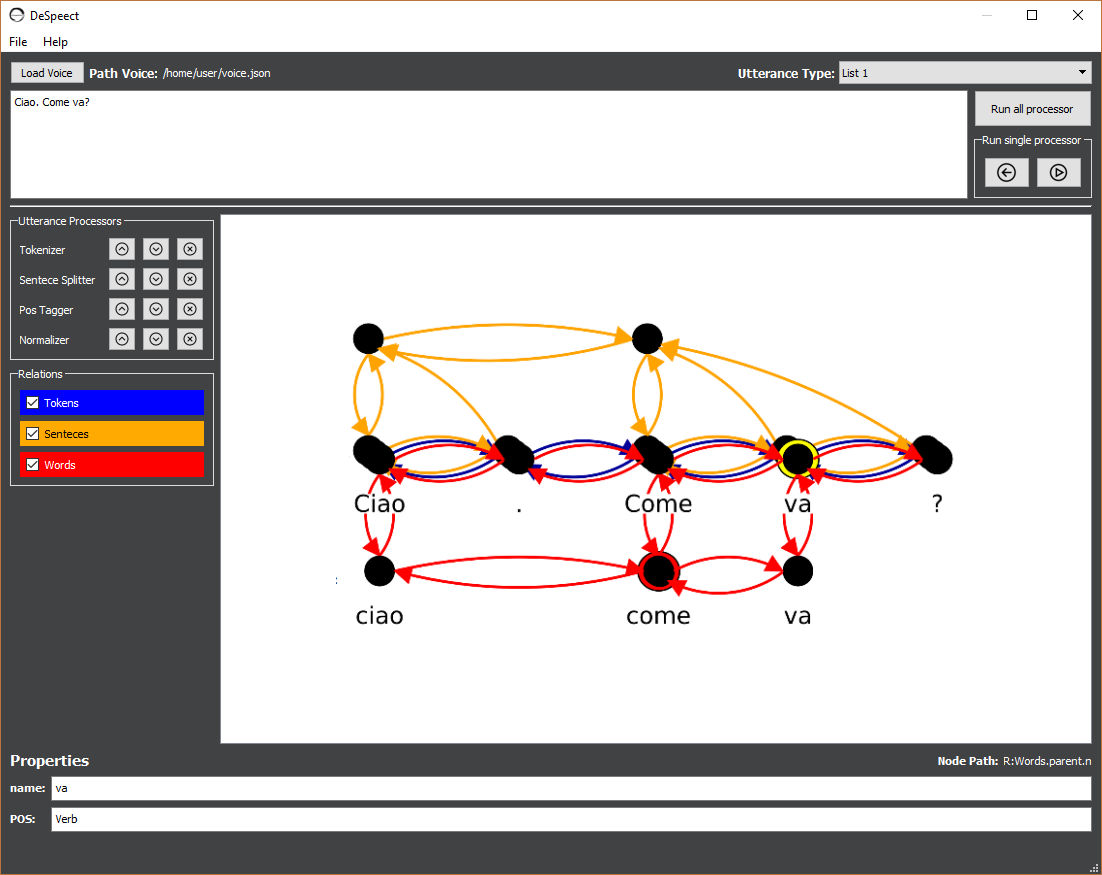
\includegraphics[width=\textwidth]{../img/paginainiziale.png}
			\label{fig:GUI}
		\end{figure}	
		Nell'interfaccia grafica saranno presenti due pulsanti per caricare il \glossario{file Voice JSon}{file voice .json}, uno in alto a sinistra di nome "Load Voice" (vedi \ref{fig:GUI}) e uno di nome "Load Voice JSon" all'interno della voce "File" nella barra del menu (vedi \ref{fig:menufile}).
		 A seguito del caricamento del file Voice Json il menù a tendina "Utterance Type" (vedi \ref{fig:GUI} in alto a destra) verrà popolato con l'elenco delle varie \glossario{utterance type}{utterance type} contenute nel file stesso. 
		 Una volta selezionata la \glossario{utterance type}{utterance type} desiderata, il programma riempirà l'elenco "Utterance Processor" (vedi \ref{fig:GUI} appena sotto a sinistra della linea orizzontale che separa la parte alta dell'applicazione dal resto) con una lista di \glossario{utterance processor}{utterance processor} contenuti nella utterance type selezionata. 
		 In seguito, l'utente potrà compilare l'area di testo sottostante il pulsante "Load Voice" (vedi \ref{fig:GUI}) con il testo che desidera mandare in elaborazione a \glossario{Speect}{Speect}.
		 Proseguendo verso destra, nella figura \ref{fig:GUI}, l'utente avrà la possibilità di eseguire tutti gli \glossario{utterance processor}{utterance processor} contenuti nella utterance type premendo il pulsante "Run all processor" (vedi \ref{fig:GUI}), in alternativa, potrà eseguirli sequenzialmente uno alla volta con la possibilità di tornare al passo precedente (vedi pulsanti contenuti nell'area nominata "Run single processor" \ref{fig:GUI}). 
		 Man mano che gli utterance processor vengono eseguiti, nell'area centrale bianca (vedi \ref{fig:GUI}) verrà disegnato il \glossario{grafo HRG}{grafo HRG}.
		 Nella sezione degli utterance processor (vedi \ref{fig:GUI}) l'utente avrà la possibilità di:
		\begin{itemize}
			\item{}decidere se visualizzare il grafo HRG di una determinata utterance mediante una spunta;
			\item{}modificare l'ordine di esecuzione delle utterance agendo sulle freccie a lato della singola utterance processor;
			\item{}rimuovere una determinata utterance processor dall'elenco e quindi dalla utterance type.
		\end{itemize}
	
		 Cliccando un nodo del grafo HRG l'utente lo evidenzierà con un cerchio di colore giallo e potrà visualizzare, nella parte inferiore dell'interfaccia grafica, le sue proprietà, tra cui il percorso del nodo.
	\begin{figure}[htp]
	\caption{Esempio voce File nella barra del menu}
	\centering
	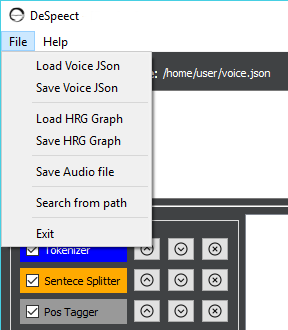
\includegraphics[]{../img/menu-file.png}
	\label{fig:menufile}
\end{figure}
	 Attraverso la voce "File" della barra del menu (vedi \ref{fig:menufile}) l'utente potrà:
	 	
		\begin{itemize}
			\item{Load Voice JSon:} caricare il file inizializzazione di Speect;
			\item{Save Voice JSon:} salvare il file inizializzazione di Speect;
			\item{Load HRG Graph:} caricare e visualizzare nell'apposita area un grafo HRG;
			\item{Save HRG Graph:} salvare lo stato di un grafo HRG;
			\item{Save Audio file:} salvare il file audio prodotto dall'esecuzione di Speect;
			\item{Search from path:} evidenziare il nodo nel grafo HRG e di conseguenza potrà vedere le sue proprietà;
			\item{Exit:} Uscire dall'applicazione.
		\end{itemize}
		 Attraverso la voce "Help" della barra del menu (vedi \ref{fig:menuhelp}) l'utente potrà:
		\begin{itemize}
			\item{Manual:} visualizzare il manuale utente;
			\item{Licence:} visualizzare la licenza di DeSpeect;
			
		\end{itemize}
	
		\begin{figure}[htp]
			\caption{Esempio voce Help nella barra di menu}
			\centering
			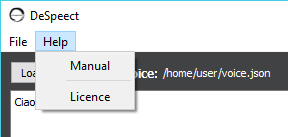
\includegraphics[]{../img/menu-help.png}
			\label{fig:menuhelp}
		\end{figure}
		
	\section{Schermata caricamento file}
	
		Mediante questa schermata (\ref{fig:filebrowser-load}) l'utente potrà navigare attraverso il \glossario{file system}{file system} e selezionare il file che desidera aprire. 
		Nell'area centrale bianca vengono visualizzati i file e le cartelle del percorso specificato nella barra "Path". Facendo doppio clic su una cartella, contenuta nel blocco centrale, verrà cambiato il percorso del "Path" e quindi verrà visualizzato il suo contenuto.
		Il primo pulsante in alto a sinistra è utilizzato per raggiungere la directory padre e visualizzarne il contenuto nell'area dedicata.
		Il pulsante in alto a destra permette all'utente di creare una nuova cartella nel percorso indicato nella barra "Path". 
		Una volta individuato il file da aprire l'utente avrà tre modi per aprirlo:
		\begin{enumerate}
			\item{} Doppio clic sopra il file;
			\item{} Un clic sopra il file e premere il pulsante "Open";
			\item{} Scrivere il nome, compreso di estensione, del file e premere il pulsante "Open".
		\end{enumerate}
		\begin{figure}[htp]
			\caption{Esempio finestra caricamento file}
			\centering
			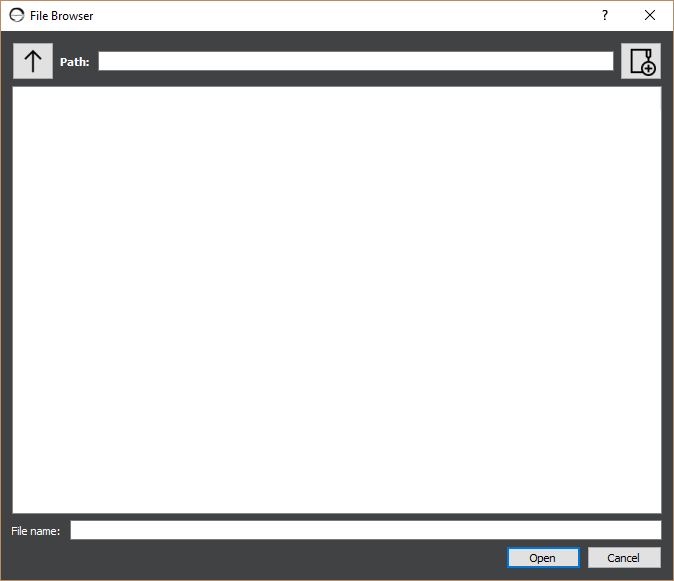
\includegraphics[width=\textwidth]{../img/filebrowser-load.png}
			\label{fig:filebrowser-load}
		\end{figure}

	\section{Schermata salvataggio file}
	
	
		Mediante questa schermata (\ref{fig:filebrowser-save}) l'utente potrà navigare attraverso il \glossario{file system}{file system} e posizionarsi all'interno della cartella nella quale vuole salvare il file.
		Nell'area centrale bianca vengono visualizzati i file e le cartelle del percorso specificato nella barra "Path". Facendo doppio clic su una cartella, contenuta nel blocco centrale, verrà cambiato il percorso del "Path" e quindi verrà visualizzato il suo contenuto.
		Il primo pulsante in alto a sinistra è utilizzato per raggiungere la directory padre e visualizzarne il contenuto nell'area dedicata.
		Il pulsante in alto a destra permette all'utente di creare una nuova cartella nel percorso indicato nella barra "Path". 
		Una volta individuato il punto in cui salvare il file bisogna:
		\begin{itemize}
			\item{} Scrivere il nome del file nell'apposito campo senza riportare l'estensione;
			\item{} Selezionare l'estensione del file;
			\item{} Premere il pulsante "Save".
		\end{itemize}
	\begin{figure}[htp]
			\caption{Esempio finestra salvataggio file}
			\centering
			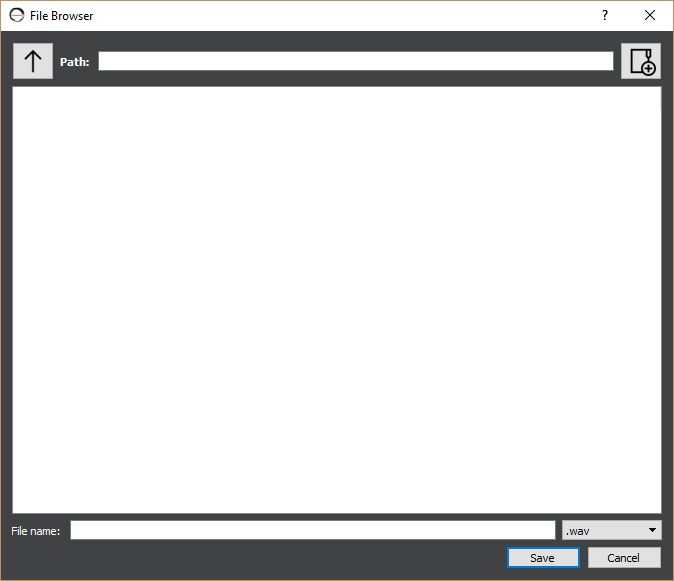
\includegraphics[width=\textwidth]{../img/filebrowser-save.png}
			\label{fig:filebrowser-save}
		\end{figure}

\end{document}